%%%%%%%%%%%%%%%%%%%%%%%%%%%%%%%%%%%%%%%%%%%%%%%%%%%%%%%%%%%%%%%%%%%%%%%%%%%%%%%%

\section{Bitcoin jako decentralizovaný finanční systém}
\label{sec_bitcoin}

Klíčovým bodem fungování Bitcoinu je veřejná distribuovaná "účetní kniha", zvaná \textit{blockchain}. V~té jsou zaznamenány všechny transakce, které kdy byly v~bitcoinové síti uskutečněny. Každý uzel disponuje svojí vlastní kopií, kterou si aktualizuje. Velmi zjednodušeně jsou transakce zapisovány následovně: z~adresy $X$ je odesláno $N$ bitcoinů na adresu $Y$. Uživatel disponuje typicky mnoha adresami, v~ideálním případě novou adresou pro každou platbu.

%%%%%%%%%%%%%%%%%%%%%%%%%%%%%%%%%%%%%%%%%%%%%%%%%%%%%%%%%%%%%%%%%%%%%%%%%%%%%%%%

\subsection{Autentizace}
\label{sec_bitcoin_autentizace}

V~systému je bezpochyby nutné autentizovat vlastníky jednotlivých mincí. To je zajištěno pomocí asymetrické kryptografie. Jednotlivé mince uživatelů jsou přiřazeny k~pseudonymům -- bitcoinovým adresám. Adresa je pouze derivátem veřejného klíče. Výhradně ten, kdo disponuje soukromým klíčem, který náleží danému veřejnému klíči, může vygenerovat validní digitální podpis. Tím se v~síti autentizuje jako vlastník mince na dané adrese a může vytvořit platnou transakci.

Protokol je navržen tak, aby každý uživatel mohl disponovat unikátní adresou pro každou svoji minci. Klíče k~jednotlivým adresám uživatelé mají uložené ve svých peněženkách. Peněženka je software pro správu klíčů a vytváření transakcí. Vytvořená transakce je zaslána konkrétnímu bitcoinovému uzlu, který, je-li transakce validní, ji zašle dalším uzlům.

%%%%%%%%%%%%%%%%%%%%%%%%%%%%%%%%%%%%%%%%%%%%%%%%%%%%%%%%%%%%%%%%%%%%%%%%%%%%%%%%

\subsection{Opětovné utracení}
\label{sec_bitcoin_opetovne_utraceni}

Opětovné utracení (\textit{replay attack}) znamená, že uživatel svoji konkrétní minci utratí vícekrát. Nic uživateli nebrání, vytvořit transakci s~validním podpisem, který utrácí minci, kterou již někdy dřívě utratil. V~systému je nutné rozpoznávat, které mince již byly utraceny a které nikoliv.

V~bitcoinovém protokolu je toto řešeno sledováním historie mincí. Jednotlivé mince řetězíme za sebe, tak jak v~jednotlivých transakcích putují napříč různými adresami. Známe tedy historii všech mincí od jejich vzniku (viz sekce~\ref{sec_bitcoin_tezeni}) až po jejich současnost -- tzv. neutracený transakční výstup (UTXO -- \textit{Unspent transaction output}). Výhradně UTXO může figurovat jako vstup transakce, tím je zajištěno, že vlastník nemůže stejnou "minci" utratit vícekrát.

\begin{figure}[ht]
    \centering
    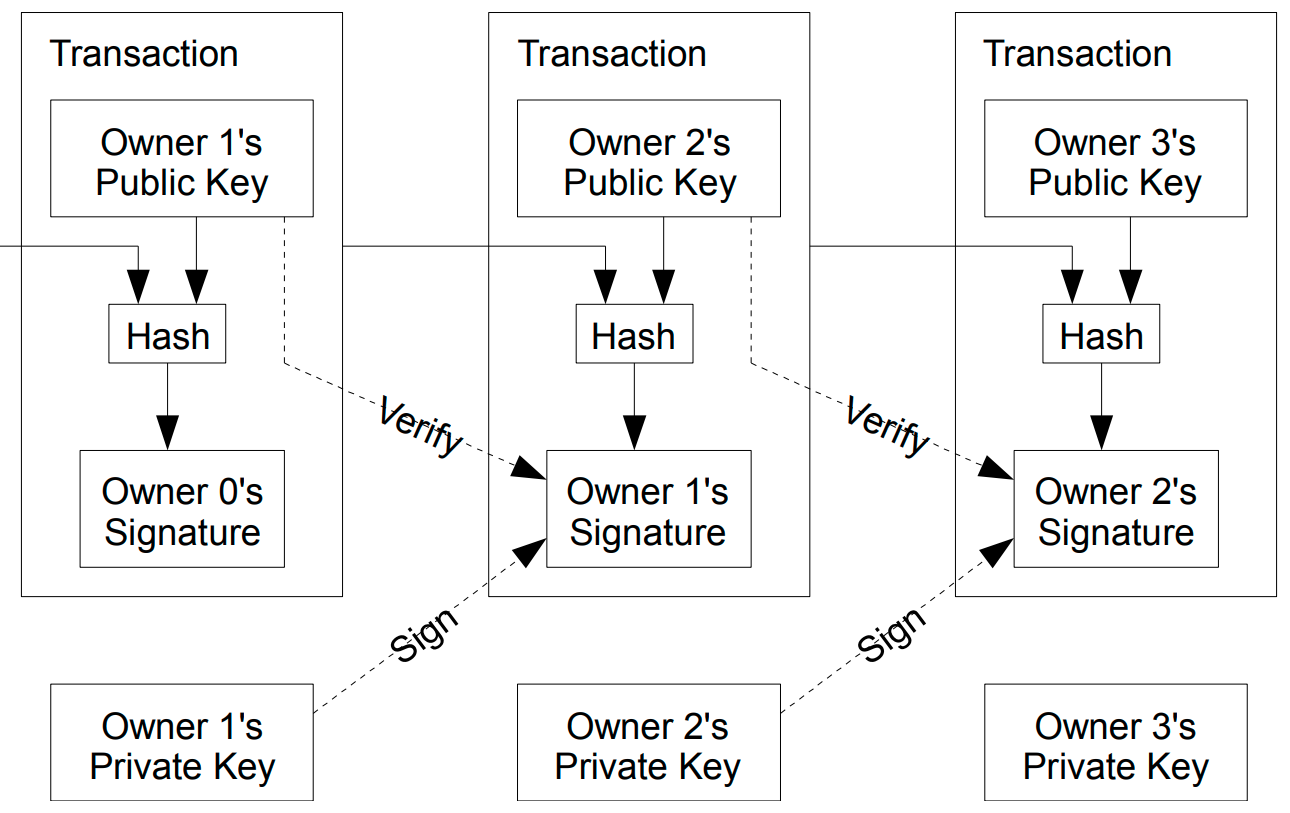
\includegraphics[width=0.75\linewidth]{transaction.png}
    \caption{Bitcoinové transakce~\cite{bib_white_paper}.}
    \label{fig_transaction}
\end{figure}

%%%%%%%%%%%%%%%%%%%%%%%%%%%%%%%%%%%%%%%%%%%%%%%%%%%%%%%%%%%%%%%%%%%%%%%%%%%%%%%%

\subsection{Dvojí utracení}
\label{sec_bitcoin_dvoji_utraceni}

Dvojí utracení (\textit{double spend attack}) je takový problém, kdy uživatel disponující UTXO $X$, vytvoří transakci, ve které utrácí UTXO $X$ na adresu $Y$ a zároveň jinou transakci, ve které utrácí UTXO $X$ na adresu $Z$. Každou transakci pošle jinému uzlu. Ten transakci zvaliduje a pošle dále do sítě. Jelikož jsme si doposud nepředstavili žádný systém časových razítek, síť není schopná vyhodnotit, která transakce je platná (byla zadána jako první) a která je neplatná (má jako vstup již utracené UTXO).

Ochrana před dvojím utracením je řešena právě \textit{blockchainem}. Transakce jsou agregovány do bloků, které jsou zhruba každých 10 minut uzavírány. Každý blok obsahuje kromě samotných transakcí také hash (SHA-256) předchozího bloku. Tím jsou bloky zřetězeny za sebe (odtud název blockchain) a vzniká chronologické uspořádání. Pokud by někdo chtěl měnit informace v~již uzavřeném bloku (blok nad kterým staví již další blok), musí přepočítat hashe všech následujících bloků\footnote{Z tohoto hlediska funguje podobným způsobem verzovací distribuovaný systém Git.}.

%%%%%%%%%%%%%%%%%%%%%%%%%%%%%%%%%%%%%%%%%%%%%%%%%%%%%%%%%%%%%%%%%%%%%%%%%%%%%%%%

\subsection{Důkaz prací}
\label{sec_bitcoin_dukaz_praci}

V~bitcoinovém protokolu je konsenzus nastaven tak, že nejdelší blockchain je pravda. V~tuto chvíli by však bylo možné změnit jakoukoliv již zapsanou transakci, přepočítat hashe všech následujících bloků a prohlásit tuto verzi blockchainu za nejdelší řetězec a tím pádem pravdu.

Abychom tomuto zamezili, musí být zápis do blockchainu nákladná operace. Toho je v~Bitcoinu docíleno tak, že na hash bloku jsou kladeny nějaké nároky. Konkrétně takové, že výsledný hash musí být malé číslo. K~tomuto účelu je v~bloku místo pro náhodné číslo, tzv. \textit{nonce}. Pokud chce někdo přidat nový blok do blockchainu, musí najít takové číslo, které způsobí, že výsledný hash bloku bude odpovídat současným nárokům sítě. Tyto nároky se v~průběhu času mění podle výpočetního výkonu celé sítě tak, aby bloky byly uzavírány v~průměru každých 10 minut.

Tento koncept se nazývá důkaz prací (z~anglického \textit{proof of work}).

\begin{figure}[ht]
    \centering
    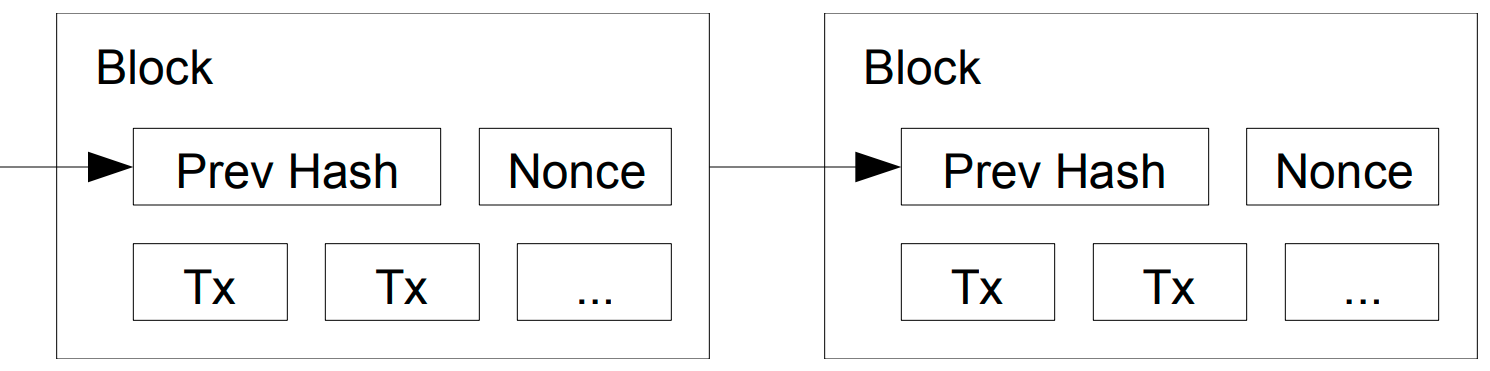
\includegraphics[width=0.75\linewidth]{blockchain.png}
    \caption{Chronologické zřetězení bloků za sebe -- \textit{blockchain}~\cite{bib_white_paper}.}
    \label{fig_blockchain}
\end{figure}

%%%%%%%%%%%%%%%%%%%%%%%%%%%%%%%%%%%%%%%%%%%%%%%%%%%%%%%%%%%%%%%%%%%%%%%%%%%%%%%%

\subsection{Těžení}
\label{sec_bitcoin_tezeni}

Proces hledání správných \textit{nonce} a zapisování nových bloků do blockchainu se nazývá těžení (\textit{Bitcoin Mining}). Entity, které tuto činnost vykonávají se nazývají těžaři (\textit{Bitcoin Miners}). Bitcoinový protokol motivuje uživatele tuto činnost provádět tak, že za uzavření bloku poskytuje odměnu v~podobě nově vzniklých bitcoinů. Ty jsou vytvořeny v~rámci tzv. \textit{coinbase} transakce, což je vždy první transakce v~bloku.

Těžař poskládá transakce dalších uživatelů do bloku, přidá hash předcházejícího bloku a generuje náhodná čísla jako potenciální \textit{nonce}. Z~toho pomocí hashovací funkce SHA-256 spočítá hash a zkontroluje, zda náhodou výsledný hash není dostatečně malé číslo. Pokud měl štěstí a je, blok je vytěžen a těžař ho rozpošle dalším uživatelům. Ti ho přijmou a začnou těžit další bloky nad ním.

Aby těžaři získávali odměnu v~pravidelných a více predikovatelných intervalech, začaly se formovat tzv. \textbf{těžařské pooly} (\textit{Mining Pool}). Několik těžařů spojí svůj výpočetní výkon a figurují jako jedna entita. Pokud některý z~nich vytěží blok, odměnu si rozdělí s~ostatními proporciálně dle jejich výpočetního výkonu.

Odměna za vytěžený blok se skládá ze dvou složek. Kromě již zmíněné \textit{coinbase} transakce s~nově vzniklými bitcoiny, dostane těžař také transakční odměny ze všech transakcí v~bloku. Uživatelé, chtějí-li motivovat těžaře, aby zahrnuli jejich transakci do bloku, platí transakční poplatky. Ty jsou definovány jako rozdíl mezi transakčními vstupy a transakčními výstupy, viz rovnice~\ref{eq_tx_fees}.

\begin{equation}
    in_1 + \ldots + in_n - out_1 - \ldots - out_m = tx\_fee
    \label{eq_tx_fees}
\end{equation}

%%%%%%%%%%%%%%%%%%%%%%%%%%%%%%%%%%%%%%%%%%%%%%%%%%%%%%%%%%%%%%%%%%%%%%%%%%%%%%%%
